 %%%  Ukázkový text a dokumentace stylu pro text závěrečné (bakalářské a
%%%  diplomové) práce na KI PřF UP v Olomouci
%%%  Copyright (C) 2012 Martin Rotter, <rotter.martinos@gmail.com>
%%%  Copyright (C) 2014 Jan Outrata, <jan.outrata@upol.cz>


%%  Pro získání PDF souboru dokumentu je třeba tento zdrojový text v
%%  LaTeXu přeložit (dvakrát) programem pdfLaTeX.

%%  V případě použití programu BibLaTeX pro tvorbu seznamu literatury
%%  je poté ještě třeba spustit program Biber s parametrem jméno
%%  souboru zdrojového textu bez přípony a následně opět (dvakrát)
%%  přeložit zdrojový text programem pdfLaTeX.

%%  Postup získání Postscriptového souboru je popsán v dokumentaci.


%%  Třída dokumentu implementující styl pro závěrečnou práci. Vybrané
%%  nepovinné parametry (ostatní v dokumentaci):

%%  'master' pro sazbu diplomové práce, jinak se sází bakalářská práce

%%  'field=kód' pro Váš studijní obor, kódy pro diplomovou práci 'uvt'
%%  pro Učitelství výpočetní techniky pro střední školy a 'binf' pro
%%  Bioinformatiku, jinak je výchozí Informatika, a pro bakalářskou
%%  práci 'ainfk' pro Aplikovanou informatiku v kombinované formě,
%%  'inf' pro Informatiku, 'infv' pro Informatiku pro vzdělávání a
%%  'binf' pro Bioinfomatiku, jinak je výchozí Aplikovaná informatika
%%  v prezenční formě

%%  'printversion' pro sazbu verze pro tisk (nebarevné logo a odkazy,
%%  odkazy s uvedením adresy za odkazem, ne odkazy do rejstříku),
%%  jinak verze pro prohlížeč

%%  'biblatex' pro zapnutí podpory pro sazbu bibliografie pomocí
%%  BibLaTeXu, jinak je výchozí sazba v prostředí thebibliography

%%  'language=jazyk' pro jazyk práce, jazyky english pro anglický,
%%  slovak pro slovenský, jinak je výchozí czech pro český

%%  'font=sans' pro bezpatkový font (Iwona Light), jinak výchozí
%%  patkový (Latin Modern)

\documentclass[
%  master,
%  field=inf,
%  printversion,
  master=true,
  biblatex,
%  language=english,
%  font=sans,
  glossaries,
  index
]{kidiplom}

%% Informace pro úvodní strany. V jazyku práce (pokud není v komentáři
%% uvedeno česky) a anglicky. Uveďte všechny, u kterých není v
%% komentáři uvedeno, že jsou volitelné. Při neuvedení se použijí
%% výchozí texty. Text pro jiný než nastavený jazyk práce (nepovinným
%% parametrem language makra \documentclass, výchozí český) se zadává
%% použitím makra s uvedením jazyka jako nepovinného parametru.

%% Název práce, česky a anglicky. Měl by se vysázet na jeden řádek.
\title{Prolamování CAPTCHA zabezpečení}
\title[english]{Breaking the CAPTCHA}

%% Volitelný podnázev práce, česky a anglicky. Měl by se vysázet na
%% jeden řádek. Výchozí je prázdný.
% \subtitle{Ukázkový text a dokumentace stylu v \LaTeX{}u}
% \subtitle[english]{Sample text and documentation of the \LaTeX{} style}

%% Jméno autora práce. Makro nemá nepovinný parametr pro uvedení
%% jazyka.
\author{Bc. Kamil Hanus}

%% Jméno vedoucího práce (včetně titulů). Makro nemá nepovinný
%% parametr pro uvedení jazyka.
\supervisor{Mgr. Martin Trnečka, Ph.D.}

%% Volitelný rok odevzdání práce. Výchozí je aktuální (kalendářní)
%% rok. Makro nemá nepovinný parametr pro uvedení jazyka.
%\yearofsubmit{\the\year}

%% Anotace práce, včetně anglické (obvykle překlad z jazyka
%% práce). Jeden odstavec!
\annotation{Ukázkový text závěrečné práce na Katedře informatiky
  Přírodovědecké fakulty Univerzity Palackého v Olomouci, který je
  zároveň dokumentací stylu pro text práce v \LaTeX{}u. Zdrojový text
  v \LaTeX{}u je doporučeno použít jako šablonu pro text skutečné
  závěrečné práce studenta.}

\annotation[english]{Sample text of thesis at the \kitextdepten,
  \kitextfacultyen, \kitextuniven{} and, at the same time,
  documentation of the \LaTeX{} style for the text. The source text in
  \LaTeX{} is recommended to be used as a template for real student's
  thesis text.}

%% Klíčová slova práce, včetně anglických. Oddělená (obvykle) středníkem.
\keywords{styl textu; závěrečná práce; dokumentace; ukázkový text}
\keywords[english]{text style; thesis; documentation; sample text}

%% Volitelná specifikace příloh textu práce, i anglicky. Výchozí je '1
%% CD/DVD'.
%\supplements{jedno kulaté placaté CD/DVD s malou kulatou dírou uprostřed}
%\supplements[english]{one round flat CD/DVD with a small round hole in the middle}

%% Volitelné poděkování. Stručné! Výchozí je prázdné. Makro nemá
%% nepovinný parametr pro uvedení jazyka.
\thanks{Děkuji, děkuji, děkuji.}

%% Cesta k souboru s bibliografií pro její sazbu pomocí BibLaTeXu
%% (zvolenou nepovinným parametrem biblatex makra
%% \documentclass). Použijte pouze při této sazbě, ne při (výchozí)
%% sazbě v prostředí thebibliography.
\bibliography{bibliografie.bib}

%% Další dodatečné styly (balíky) potřebné pro sazbu vlastního textu
%% práce.
\usepackage{lipsum}
\usepackage{verbatimbox}

\begin{document}
%% Sazba úvodních stran -- titulní, s bibliografickými údaji, s
%% anotací a klíčovými slovy, s poděkováním a prohlášením, s obsahem a
%% se seznamy obrázků, tabulek, vět a zdrojových kódů (pokud jejich
%% sazba není vypnutá).
\maketitle

%% Vlastní text závěrečné práce. Pro povinné závěry, před přílohami,
%% použijte prostředí kiconclusions. Povinná je i příloha s obsahem
%% přiloženého CD/DVD.

%% -------------------------------------------------------------------

\newcommand{\BibLaTeX}{\textsc{Bib}\LaTeX}
\renewcommand\UrlFont{}



\section{Úvod}
V posledních letech urazila technologie strojového učení a umělé inteligence velký posun vpřed. Ačkoliv historie vzniku termínu strojové učení sahá do  60. let 20. století, masová adaptace nastává až v posledních několika letech, kdy se lze s pojmy umělá inteligence či AI (z anglického \textit{artificial intelligence} \footnote{\url{https://trends.google.com/trends/explore?date=all\&q=\%2Fm\%2F01hyh\_}}. Můžeme se domnívat, že jistou spojitost s nárůstem zájmu o strojové učení má i zpřístupnění open-source nástrojů, umožňujících snadnou aplikaci příslušných algoritmů, široké veřejnosti \footnote{\url{https://trends.google.com/trends/explore?date=all\&q=\%2Fm\%2F01hyh\_,\%2Fg\%2F11gd3905v1,\%2Fg\%2F11bwp1s2k3,\%2Fg\%2F11c1r2rvnp}}.

Cílem této diplomové práce je  rozšíření autorových znalostí v oblasti umělé inteligence. Jako vhodný problém na kterém lze demonstrovat potenciál strojového učení se naskýtá prolamování CAPTCHA zabezpečení. Aktuálně dostupné nástroje strojového učení poskytují elegantní způsob jak prolamovat klasické CAPTCHA zabezpečení. Zřejmě proto lze pozorovat vývoj nových typů CAPTCHA zabezpečení, které využívají některé prvky umělé inteligence. Diplomovou práci lze rozdělit do dvou částí -- první se zabývá samotným problémem CAPTCHA zabezpečení, jeho historií a možným prolamováním. Druhá popisuje aplikaci nazvanou CaptchaBreaker, která popisuje možnost jak lze v rozumném čase řešit problém dekódování některých typů CAPTCHA kódů.
\newpage
\section{Captcha}
\subsection{Historie}
Za akronymem CAPTCHA stojí anglický text \uv{\textbf{C}ompletely \textbf{A}utomated \textbf{P}ublic \textbf{T}uring test to tell \textbf{C}omputers and \textbf{H}umans \textbf{A}part}. Obecně je principem tohoto testu vygenerování určitého typu dotazu a ověření odpovědi, typicky na webových stránkách. Na základě verifikace odpovědi je rozhodnuto, zda systém komunikuje s reálným uživatelem nebo robotem. Některé zdroje uvádějí [česká wiki] pouze přepis textu z deformovaného obrazu do vstupního pole, což lze považovat za zavádějící, jelikož existuje mnoho dalších  variant. 

Důvod pro zavedení takové ochrany je prostý. Pokud je umožněno na web zaslat libovolné požadavky bez omezení (například. příspěvky do diskuzních fór, zakládání uživatelských účtů, pokusy o přihlášení, atd.), lze očekávat že takové příležitosti využije útočník a začne systém zahlcovat, možná s úmyslem zamezit přístupnosti či šíření spamu. Ovšem je nutné mít na paměti, že nutnost ověřovat svou autentičnost je pro uživatele snížením komfortu. Proto se objevují technologie které během prvotní interakce nepožadují ověření žádné, nebo ověřují uživatele natolik sofistikovanými metodami, že není nutná jeho	 interakce.


Zajímavým použitím technologie byla digitalizace archivu článků deníku The New York Times či literárních děl společností Google. Slova, která nebylo možné strojově rozpoznat s dostatečnou přesností byla dekódována s použitím nástroje reCAPTCHA. Metoda spočívala vždy v zobrazení obrázků dvou slov v kódu, přičemž u jednoho z nich byl známý jeho obsah. Pokud uživatel zadal správně známou část, o druhé také uvažovalo že je zadaná správně. Samozřejmě takové řešení by bylo příliš naivní a proto lze usuzovat, že za popsaným procesem existuje ještě další ověřovací mechanismus, který porovnává odpovědi uživatelů pro konkrétní slova a přiřadí jim váhu dle jejich výskytu. 
\subsection{Druhy kódů}
https://dynomapper.com/blog/514-online-captcha-solving-services-and-available-captcha-types
https://ai.google/research/pubs/pub43464
 - textová, obrázková, audio, noCaptcha, aka slider na binance, přihlášení přes sociální media (bot nemá účet), honeypot (skryté fieldy, človek nevidí, bot ano a tak je vyplní)
 
\subsubsection*{Leetspeak} 
Na úvod je vhodné zmínit tzv. \textit{leetspeak} kódy. V raných fázích internetu se jednalo o přepis znaků, které s užitím jisté míry představivosti tvořily smysluplný text (např. \textit{N04m} jako ekvivalent slova \textit{Noam}), avšak pro útočníka bez znalosti generujícího mechanismu bylo obtížné automatizovat vyplňování kontrolních otázek. Takové ověření bylo možné potkat např. na některých IRC(odkaz co to je) kanálech [zdroj].
 
\subsubsection*{Jednoduchá otázka}
Velmi triviální metodou, kterak lze implementovat CAPTCHA zabezpečení, je použít jednoduchou textovou hádanku. Jedná se například o otázku typu \textit{Jaký je dnes den?} očekávající na vstupu jednoslovný název dne v týdnu. Obdobně lze hovořit o jednoduchých matematických otázkách \textit{Kolik je 4 krát 6?}. V případě, že není použit sofistikovaný nástroj generující nové druhy otázek je řešení tohoto zabezpečení triviální. Vyvine-li útočník dostatečné úsilí, po několika vygenerování různých otázek lze popsat gramatiku CAPTCHA schématu. Naivním řešením je zkonstruovat mapovací tabulku jednotlivých slov na funkce, se navzájem aplikují. Vzhledem ke konečnosti generovaných výrazů je však možné, že vytvoření formální gramatiky popisující jazyk CAPTCHA schématu a následné vytvoření překladače by mělo větší úspěšnost. Vzhledem k velmi nízkému rozšíření (odkaz) tohoto typu zabezpečení však lze usuzovat, že takové usilí vyvine zanedbatelný počet útočníků. (přesunout možnost prolomení do jiné kapitoly)

\subsubsection*{Zkreslený text}
Stále běžně se vyskytujícím typem CAPTCHA zabezpečení je přepis textu z deformovaného obrazu uživatelem. Předpokládá se, že bot není schopný vlivem zkreslení provést extrakci jednotlivých symbolů z obrazu. Ztížit čtení obrazu je možné mnoha způsoby - rozostřením textu, spojením jednotlivých znaků, vložením zkreslujících křivek, vynecháním malých částí znaků, atd. V další kapitole se diplomová práce zaměřuje právě na možnost prolomení typů CAPTCHA využívají zkreslování textu v obraze.

\begin{figure}
  \centering
  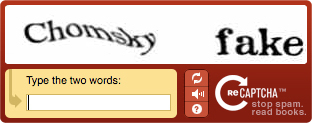
\includegraphics[scale=0.8]{images/text_image_captcha.jpg}
  \caption{Příklad obrázku, které generovala služba reCAPTCHA (verze 1) obsahující text \uv{Chomsky fake}.}
  \label{fig:captcha_text_image}
\end{figure}


\subsubsection*{Identifikace objektů v obraze}
Uživatelsky komfortnějším přístupem, jak rozlišit člověka od počítače, je zobrazit uživateli množinu různých obrázků a požadovat výběr pouze těch, které obsahují nějaký předmět. Zaměříme-li se na technologii Google reCaptcha [odkaz], lze pozorovat dva přístupy k tomuto problému. První variantou je zobrazit uživateli 9 obrázků, ze kterých je například vyžadován výběr pouze těch obsahujíce dopravní značky. Druhý přístup je segmentace obrazu do několika částí a vyžadování výběru pouze těch, které obsahují určitý objekt (například auto). Využití využití podobného přístupu se také využívá k monetizaci obsahu majitelů webů, jelikož existují technologie [odkaz] používající CAPTCHA jako inzertní plochu. 

\begin{figure}
  \centering
  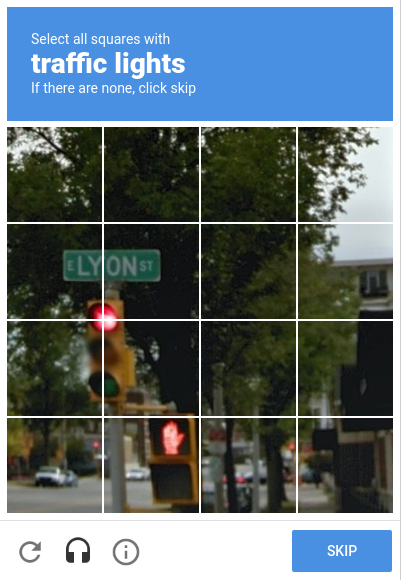
\includegraphics[scale=0.8]{images/squares.png}
  \caption{Varianta reCAPTCHA v2, kde má uživatel vybrat všechny dlaždice obsahující semafor.}
  \label{fig:captcha_geetest}
\end{figure}

\subsubsection*{Skládání puzzle}
Další variantou CAPTCHA technologie pracující s obrazem nazvěme skládáním puzzle (společnost \textit{GeeTest} \ref{fig:captcha_geetest} používá anglický název \uv{slide}). Přístup spočívá spočívá v přesunu části obrazu ve tvaru dílku puzzle zpět na své původní místo pomocí posuvníku. Během procesu ověření je sledováno několik faktorů ovlivňujících vyhodnocovací proces, například doba posuvu, cesta myši, doplňky prohlížeče. 

\begin{figure}
  \centering
  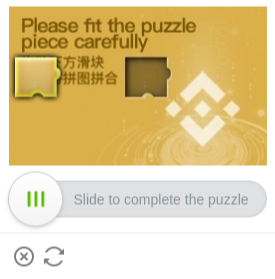
\includegraphics{images/geetest.png}
  \caption{Varianta GeeTest CAPTCHA používaná na webu \url{binance.com}}
  \label{fig:captcha_geetest}
\end{figure}


\subsubsection*{Audio CAPTCHA}
Zabezpečení pomocí textové/obrazové kontrol má nevýhodu v tom, že velmi limituje uživatele se zrakovým postižením, kteří například vnímají odlišně barevné spektrum. Právě proto je vhodné jako sekundární možnost nabídnout tzv. audio CAPTCHA zabezpečení, jehož princip spočívá v přepisu znaků které jsou vloženy do audio záznamu. I zde lze najít různé typy zkreslení zvuku, které zvyšují obtížnost dekódování nahrávky. 

\subsection{Možnosti prolamování}
 \subsubsection{Strojové učení}
 - NN a CNN
\newpage
\section{Captcha Breaker}
Cílem diplomové práce bylo demonstrovat možnosti prolamování CAPTCHA zabezpečení, přičemž hlavní inspirace pocházela z textu \texttt{How to Mimic Humans, Guide for Computers}. Byly vybrány různé typy zabezpečení, které ověřují rozpoznání zkresleného textu v obraze. S ohledem na odlišný postup rozpoznání segmentovaných částí obrazů byly prolamovány některé shodné typy zabezpečení. 

Výsledná aplikace se skládá ze dvou částí -- algoritmu rozpoznávajícího různé typy CAPTCHA zabezpečení a webové aplikace, která umožňuje pohodlnou tvorbu datasetu, klasifikátoru a umožňuje prolomit známá schémata.


\subsection{Použité technologie}
\subsubsection*{Python}

\subsubsection*{Flask}
Flask je microframework určený pro tvorbu webových aplikací napsaný v jazyce Python. Samotné jádro frameworku v základu obsahuje s nadsázkou pouze nástroje pro směrování požadavků a šablonovací systém Jinja. Vyžadujeme-li funkcionalitu navíc, jako například práci s DB, ORM mapování, validaci formulářů nebo autentizaci požadavků, je nutné doinstalovat patřičný modul. Framework se tedy snaží být minimalistický a je pouze na uvážení vývojáře, jaké moduly ke strohému jádru dodá. 
\subsubsection*{PostgreSQL}
Pro perzistentní uložení informací bylo nutné zvolit některý z relačních databázových enginů. V tomto případě padla volba na PostgreSQL, což je open-source relační SQL databáze. Stejně tak by pro potřeby projektu byla vyhovující jakýkoliv Flaskem podporovaný engine, například MariaDB nebo MySQL.
\subsubsection*{Celery}
Důležitým vlastností pro některé aplikace je možnost vykonávat některé operace asynchronně. K tomu lze v případě Flasku použít například Celery. Jedná se distribuovaný systém sloužící pro zpracování zasílaných zpráv, které předávány skrze nějakého z podporovaných prostředníků, tzv. brokerů. I když primárně míří na zpracování v reálném čase, podporuje například zařazení obdržených zpráv do fronty a jejich sekvenční zpracování.

Chceme-li vytvořit nějakou metodu, kterou bude možné v pythonu spustit asynchronně, je nutné obalit ji dekorátorem \texttt{@celery.task}. Tím je umožněno instanci Celery workeru vyhledat všechny tasky v dané aplikaci a uložit si je do paměti. Obdrženou zprávu lze poté chápat jako dvojici \texttt{název metody}-\texttt{argumenty}. Pracujeme-li s databázovými objekty, je možné k jejich předávání přistoupit dvěma způsoby. Buď jako argument předáme ID objektu a v metodě samotné je objekt načítán z databáze a nebo předáme jako argument objekt samotný, který je následně serializován před zasláním zprávy.

\subsubsection*{Redis}
Jako broker pro komunikaci s Celery byl použit Redis. Jedná se o úložiště pracující primárně v operační paměti, nicméně lze jej nakonfigurovat tak, aby ukládal data na pevný disk a po restartu zařízení byl schopen obnovit svůj stav.

\subsubsection*{jQuery}
jQuery je již několik let nejpoužívanější javascriptovou knihovnou \footnote{$https://w3techs.com/technologies/overview/javascript_library/all$} vůbec. Mezi její silné stránky patří snadná manipulace s DOM nebo tvorba AJAX requestů. Těchto vlastností využívá zejména průvodce tvorbou datasetu v administrační části aplikace.
\subsubsection*{Bootstrap}
Spolu s jQuery tvoří CSS knihovna Bootstrap základ velkého množství webů. Programátor je s jejím použítím odstíněn od nutnosti stylovat prvky webové stránky a je možné se více soustředit na samotný vývoj backendu.
\subsubsection*{PyTorch}
Open-source knihovna zaměřená na strojové učení v jazyce Python. 


\subsection{Prolamované typy}
 
\begin{itemize}
	\item \textbf{adiseet.mfcr.cz} - Daňový portál Finanční správy České republiky. 
	\item \textbf{kamody.cz} - Typický příklad e-shopu s nevyhovujícím zabezpečením.
	\item \textbf{mojedatovaschranka.cz} - Portál určený pro elektronickou komunikaci s úřady. \footnote{V průběhu tvorby diplomové práce došlo k zásadní aktualizaci webové aplikace \texttt{mojedatovaschranka.cz} a původní CAPTCHA zabezpečení bylo nahrazeno technologií Google reCAPTCHA.}
	\item \textbf{telerik.com} - Domovská stránka frameworku pro ASP.NET, který využívají miliony webů.
	\item \textbf{ulozto.cz} - Populární služba pro sdílení souborů.
\end{itemize}


\subsection{Extrakce symbolů}
\subsubsection{Podporované grafické operace}
\begin{itemize}
\item 
\end{itemize}
\subsection{Uživatelská část}
Část aplikace, která je dostupná široké veřejnosti, lze rozdělit do dvou skupin -- prezentace známých schémat a API. Domovská stránka seznamuje uživatele zejména s účelem projektu a dává mu možnost vyzkoušet si prolamování CAPTCHA obrázků v praxi. Po výběru obrázku k prolomení a příslušného klasifikátoru je možné zaslat dotaz na server, který z obrázku dekóduje znaky pomocí vybraného klasifikátoru, což je řešeno asynchronním dotazem na API rozhraní. Nastane-li chyba, je uživateli zobrazena příslušná hláška. V případě úspěšného rozpoznání pouze obsah zaslaného obrázku.\\

API obsahuje pouze jednu cestu, na kterou se zasílá POST request se dvěma parametry -- ID klasifikátoru a obrázek zakódovaný do Base64. Jakmile server obdrží požadavek, nejprve zkontroluje existenci klasifikátoru. Pokud přijal špatnou hodnotu, informuje o tom v odpovědi. Následně dekóduje obrázek, zjistí jeho formát (jpeg, png, gif, etc..) a normalizuje jej do podoby kterou akceptuje klasifikátor, resp. příslušný proces extrakce symbolů.

\begin{minipage}{0.45\textwidth}
\begin{verbatim}
{
"message":
"Unknown classifier",
"status":
"error"
}
\end{verbatim}
Chybová odpověď
\end{minipage}
\hfill
\begin{minipage}{0.45\textwidth}
\begin{verbatim}
{
"message":
"10487",
"status":
"success"
}
\end{verbatim}
Odpověď v případě rozpoznání znaků
\end{minipage}

\begin{table}
\begin{tabular}{|l|l|l|}
\hline
\textbf{URL} & \textbf{metoda} & \textbf{parametry}
\\ \hline
\texttt{/} & \texttt{GET} & -
\\ \hline
\texttt{/decode/} & \texttt{POST} & image, classifier ID
\\ \hline
\end{tabular}
\caption{URL endpointy pro globální namespace}
\end{table}

\subsection{Administrační rozhraní}
Část webu dostupná pouze administrátorovi je dostupná na URL \texttt{/admin}. Všechny dotazy přicházející na adresy v tomto jmenném prostoru musejí být autentizovány. Jelikož se nepředpokládá užívání aplikace více administrátory, jsou údaje poskytnuté na přihlašovací stránce kontrolovány pouze vůči hodnotám \texttt{APP\_USERNAME} a \texttt{APP\_PASSWORD} v konfiguračním souboru. Bezpečnost takového přístupu lze dále zvýšit například restrikcí IP adres u dotazů přicházející na tyto adresy v konfiguraci použitého aplikačního serveru.

\subsubsection*{Nahrání datasetu \texttt{/admin/datasets/new/}}
Proces nahrání datasetu obsahuje konfigurátor vytvořený pomocí knihoven jQuery a  Bootstrap. Administrátor je nejprve vyzván k vybrání ZIP archivu se vzorovými CAPTCHA obrázky. Následně je mu umožněno označit nahrané obrázky texty, které obsahují. V posledním kroku je konfigurátor operací, díky nimž je možné zadefinovat pro nahrané schéma postup odstranění šumu pro extrahování symbolů. Dostupné jsou zejména tzv. morfologické operace, nicméně aplikace je navržena univerzálně a po vytvoření nové třídy reprezentující operaci dědící z třídy \texttt{AbstractOperation} je možné výběr rozšířit. Jakmile je administrátor spokojený s výsledkem, odešle dataset na server a je přesměrován na stránku s jeho detaily.
\subsubsection*{Zobrazení datasetu \texttt{/admin/datasets/:id/}}
Jakmile je dataset nahrán na server, je administrátor přesměrován na stránku s jeho detaily. V horním řádku stránky jsou informace o času vytvoření, znaky obsažené v datasetu a celkový počet rozpoznaných symbolů. Následuje výpis nahraných obrázků spolu se zobrazením extrahovaných symbolů. V poslední části je vypsána konfigurace extraktoru ve formátu JSON. 

\subsubsection*{Tvorba klasifikátoru \texttt{/admin/classifiers/new/}}
Formulář konfigurace klasifikátoru je parametrizován čtyřmi vstupy - název klasifikátoru, maximální počet iterací, cílová hodnota ztrátové funkce a zdrojový dataset. Po odeslání požadavku na vytvoření klasifikátoru je samotná fáze trénování spuštěna na pozadní a administrátor je přesměrován na nástěnku, kde vidí průběh trénování.

\subsubsection*{Detaily klasifikátoru \texttt{/admin/classifier/:id/}}
Stránka zobrazující detaily klasifikátoru v současné době zobrazuje informace z fáze učení klasifikátoru. Tedy kromě názvu klasifikátoru a zvoleného datasetu jde o výslednou hodnotu ztrátové funkce a stav fáze učení klasifikátoru. Kromě toho je možné již nahraný dataset odstranit.

\subsubsection*{Nástěnka \texttt{/admin/overview/}}
Jelikož se prvky nástěnky odkazují na pojmy vyjmenované výše, je popis domovské stránky administrátora až poslední. Na nástěnce jsou zobrazeny statistiky příchozích dotazů na rozpoznání CAPTCHA obrázků a počtu datasetů, resp. klasifikátorů. Existují-li navíc klasifikátory, které se momentálně trénují, jsou na nástěnce zobrazeny informace o stavu procesu. Kromě názvu klasifikátoru se jedná o pořadí současné iterace fáze učení nebo aktuální hodnotu ztrátové funkce. Tyto informace se pravidelně obnovují každých 5 sekund po asynchronním vyžádání detailů. Jakmile je klasifikátor natrénován, záznam z nástěnky zmizí.

\begin{table}[h]
\begin{tabular}{|l|l|l|}
\hline
\textbf{URL} & \textbf{metoda} & \textbf{parametry}
\\ \hline
\texttt{/} & \texttt{GET} & -
\\ \hline
\texttt{/overview/} & \texttt{GET} & -
\\ \hline
\texttt{/datasets/} & \texttt{GET} & -
\\ \hline
\texttt{/datasets/new/} & \texttt{GET, POST} & - 
\\ \hline
\texttt{/datasets/new/preview} & \texttt{POST} & image, operations
\\ \hline
\texttt{/datasets/:id/} & \texttt{GET} & -
\\ \hline
\texttt{/datasets/:id/delete/} & \texttt{POST} & -
\\ \hline
\texttt{/classifiers/} & \texttt{GET} & -
\\ \hline
\texttt{/classifiers/new/} & \texttt{GET, POST} & - 
\\ \hline
\texttt{/classifiers/:id/} & \texttt{GET} & -
\\ \hline
\texttt{/classifiers/:id/delete/} & \texttt{POST} & -
\\ \hline
\texttt{/task\_status/:id/} & \texttt{GET} & -
\\ \hline
\end{tabular}
\caption{URL endpointy pro namespace \texttt{/admin/}}
\end{table}


\subsection*{Další vývoj}
Jak je patrné již z popisu aplikace, k vytvoření ultimativního nástroje pro lámání CAPTCHA kódů, byť pouze obrázkových, vede ještě dlouhá cesta. Implementace následujících funkcionalit, zejména v administračním rozhraní, by výrazně zlepšila komfort užívání a zřejmě i praktičnost systému jako celku.

\begin{itemize}
\item \textbf{Upozornění na chybně klasifikované znaky.} Na stránce zobrazující detaily klasifikátoru se naskýtá možnost zobrazit chybně klasifikované obrázky. Taková chyba může nastat zejména v následujících třech případech: 1) Příliš podobné znaky (číslice nula versus písmeno O). 2) Algoritmus pro extrakci symbolů na výstupu nevrátí celý znak, ale např. pouze jeho část. 3) Symbol byl ručně chybně označen a klasifikátor jej rozpoznává správně.
\item \textbf{Změna označení již nahraných obrázků.} Během procesu vytváření datasetu musí administrátor nahrát ZIP archiv obsahující obrázky jejichž název odpovídá CAPTCHA kódu, nebo je procesem označení obrázků proveden před uploadem na server. V obou případech však závisí jen a pouze na lidském faktoru, zda bude obrázku přiřazen chybný text. To je například poslední bod předchozího odstavce. Z toho důvodu je vhodné umožnit změnu označení obrázku, resp. samotného symbolu.
\item \textbf{Odstranění některých znaků}. Druhá chyba z prvního odstavce popisuje nesprávné rozpoznání symbolu v CAPTCHA obrázku. Tomu je možné předejít úpravou parametrů extraktoru, což však může mít za následek horší rozpoznávací schopnosti symbolů v datasetu jako celku. Abychom zamezili trénování klasifikátoru na chybných datech, je vhodnější poskytnout možnost odebrat jednotlivé symboly z datasetu, které byly špatně rozpoznány. Přímý důsledek tohoto řešení je nutná úprava procesu trénování klasifikátoru CNN, resp. hodnoty udávající počet současně zpracovávaných vstupů.
\item  \textbf{Volba z více klasifikátorů.} V současné době systém používá jako klasifikátor konvoluční neuronovou síť se dvěma konvolučními vrstvami, kde se na každý vstup uplatní funkce \texttt{MaxPool} s velikostí jádra = 2. To nemusí vyhovovat všem rozpoznávaným instancím CAPTCHA obrázků a i pro účely porovnání efektivnosti klasifikátorů je rozumné přidat další a mít možnost volby. 
\item \textbf{Volba tvaru jádra morfologických operací.} Každá morfologická operace potřebuje dva vstupy - obrázek a jádro. Tvar, resp. hodnota matice, jádra má přímý vliv na výsledný obrázek. Aplikace parametrizuje jádro pouze jednou celočíselnou hodnotou udávající velikost čtvercové jednotkové matice. Je však možné použít jádro ve tvaru tzv. kříže, resp. elipsy. Příklad lze vidět na obrázku níže.
\item \textbf{Klasifikátor používající více datasetů.} K dalšímu zlepšení rozpoznávání by mohlo také vést trénování klasifikátoru znaky z více zdrojů. Kromě primárního datasetu, který udává i proces extrakce symbolů, by k jeho množině znaků byly přidány ty symboly s odpovídající hodnotou ze zvolených datasetů. Tím by se docílilo rozpoznání transformací, které v trénovací množině symbolů nebyly prve zahrnuty.
\end{itemize}


Otázky\\
\begin{itemize}
\item n-fold u klasifikátoru? s tím souvisí úspěšnost klasifikátoru
\item experimentální porovnání -- nn vs cnn, rozpoznání na úrovni obrázků vs znaků
\item počet stran práce
\item u datasetu zobrazit pokrytí jednotlivých symbolů
\item paginace obrázků datasetu

\end{itemize}

%% Závěry práce. V jazyce práce a anglicky. Text pro jiný než
%% nastavený jazyk práce (nepovinným parametrem language makra
%% \documentclass, výchozí český) se zadává použitím makra s uvedením
%% jazyka jako nepovinného parametru.
\begin{kiconclusions}
Závěr práce v \uv{českém} jazyce.
\end{kiconclusions}

\begin{kiconclusions}[english]
Thesis conclusions in \uv{English}.
\end{kiconclusions}

%% Přílohy obsahu textu práce, za makrem \appendix.
\appendix

\section{První příloha}
Text první přílohy

\section{Druhá příloha}
Text druhé přílohy

%% Obsah přiloženého CD/DVD. Poslední příloha. Upravte podle vlastní
%% práce!
\section{Obsah přiloženého CD/DVD} \label{sec:ObsahCD}

Na samotném konci textu práce je uveden stručný popis obsahu
přiloženého CD/DVD, tj.~jeho závazné adresářové struktury, důležitých
souborů apod.

\begin{description}

\item[\texttt{bin/}] \hfill \\
  Instalátor \textsc{Instalator} programu, popř.~program
  \textsc{Program}, spustitelné přímo z~CD/DVD. / Kompletní adresářová
  struktura webové aplikace \textsc{Webovka} (v~ZIP archivu) pro
  zkopírování na webový server. Adresář obsahuje i~všechny runtime
  knihovny a~další soubory potřebné pro bezproblémový běh instalátoru
  a~programu z~CD/DVD / pro bezproblémový provoz webové aplikace na
  webovém serveru.

\item[\texttt{doc/}] \hfill \\
  Text práce ve formátu PDF, vytvořený s~použitím závazného stylu KI
  PřF UP v~Olomouci pro závěrečné práce, včetně všech příloh,
  a~všechny soubory potřebné pro bezproblémové vygenerování PDF
  dokumentu textu (v~ZIP archivu), tj.~zdrojový text textu, vložené
  obrázky, apod.

\item[\texttt{src/}] \hfill \\
  Kompletní zdrojové texty programu \textsc{Program} / webové aplikace
  \textsc{Webovka} se všemi potřebnými (příp.~převzatými) zdrojovými
  texty, knihovnami a~dalšími soubory potřebnými pro bezproblémové
  vytvoření spustitelných verzí programu / adresářové struktury pro
  zkopírování na webový server.

\item[\texttt{readme.txt}] \hfill \\
  Instrukce pro instalaci a~spuštění programu \textsc{Program}, včetně
  všech požadavků pro jeho bezproblémový provoz. / Instrukce pro
  nasazení webové aplikace \textsc{Webovka} na webový server, včetně
  všech požadavků pro její bezproblémový provoz, a~webová adresa, na
  které je aplikace nasazena pro účel testování při tvorbě posudků
  práce a~pro účel obhajoby práce.

\end{description}

Navíc CD/DVD obsahuje:

\begin{description}

\item[\texttt{data/}] \hfill \\
  Ukázková a~testovací data použitá v~práci a~pro potřeby testování
  práce při tvorbě posudků a~obhajoby práce.

\item[\texttt{install/}] \hfill \\
  Instalátory aplikací, runtime knihoven a~jiných souborů potřebných
  pro provoz programu \textsc{Program} / webové aplikace
  \textsc{Webovka}, které nejsou standardní součástí operačního
  systému určeného pro běh programu / provoz webové aplikace.

\item[\texttt{literature/}] \hfill \\
  Vybrané položky bibliografie, příp.~jiná užitečná literatura
  vztahující se k~práci.

\end{description}

U~veškerých cizích převzatých materiálů obsažených na CD/DVD jejich
zahrnutí dovolují podmínky pro jejich šíření nebo přiložený souhlas
držitele copyrightu. Pro všechny použité (a~citované) materiály,
u~kterých toto není splněno a~nejsou tak obsaženy na CD/DVD, je uveden
jejich zdroj (např.~webová adresa) v~bibliografii nebo textu práce
nebo v souboru \texttt{readme.txt}.

%% -------------------------------------------------------------------

%% Sazba volitelného seznamu zkratek, za přílohami.
\printglossary

%% Sazba povinné bibliografie, za přílohami (případně i za seznamem
%% zkratek). Při použití BibLaTeXu použijte makro
%% \printbibliography. jinak prostředí thebibliography. Ne obojí!

%% Sazba i v textu necitovaných zdrojů, při použití
%% BibLaTeXu. Volitelné.
\nocite{*}
%% Vlastní sazba bibliografie při použití BibLaTeXu.
\printbibliography

%% Bibliografie, včetně sazby, při nepoužití BibLaTeXu.
% \begin{thebibliography}{9}
%\bibitem{kniha2} \uppercase{Hawke}, Paul. NanoHttpd: Light-weight HTTP server designed for embedding in other applications. GitHub [online]. 2014-05-12. [cit. 2014-12-06]. Dostupné z: \url{https://github.com/NanoHttpd/nanohttpd}
%
%\bibitem{jeske13} \uppercase{Jeske}, David; \uppercase{Novák}, Josef. Simple HTTP Server in \csharp: Threaded synchronous HTTP Server abstract class, to respond to HTTP requests. CodeProject: For those who code [online]. 2014-05-24. [cit. 2014-12-06]. Dostupné z: \url{http://www.codeproject.com/Articles/137979/Simple-HTTP-Server-in-C}
%
%\bibitem{uzis2012} \uppercase{ÚSTAV ZDRAVOTNICKÝCH INFORMACÍ A STATISTIKY ČR}. Lékaři, zubní lékaři a farmaceuti 2012 [online]. Praha 2, Palackého náměstí 4: Ústav zdravotnických informací a statistiky ČR, 2012 [cit. 2014-12-06]. ISBN 978-80-7472-089-5. Dostupné z: \url{http://www.uzis.cz/publikace/lekari-zubni-lekari-farmaceuti-2012}
% \end{thebibliography}

%% Sazba volitelného rejstříku, za bibliografií.
\printindex

\end{document}
